%\noindent

Although any statistically significant deviation in data from the  Standard Model(SM) predictions would be a manifestation of a BSM physics, the question is what we can learn about its scale and its strength before discovering new particles. The appropriate tool for answering this question is the Effective Field Theory(EFT) approach: the information about the  scale $\Lambda$ and the strength $C$ of new physics is encoded in  the Wilson coefficients of the higher dimension operators, $f_i=C^m/\Lambda^n$.
The usefulness of any EFT analysis of a given process relies on the assumption that only a few higher-dimension terms 
in the expansion ${\cal L}={\cal L}_{SM}+\sum_i f_i^{(6)}{\cal O}_i^{(6)}+ \sum_i f_i^{(8)}{\cal O}_i^{(6)}+\ldots$ 
provide adequate approximation to an unknown UV completion.   
This assumption  introduces a strong model-dependent aspect and therefore it is convenient to introduce the concept of EFT ``models" defined by the choice of operators  and the values of their Wilson coefficients $({\cal O}_i^{(d)},f_i^{(d)})$.  Our focus is on the proper use of the EFT "models" in their range of validity for the WW scattering in purely leptonic W decay channels where the $WW$ invariant mass cannot be determined experimentally. A full explanation of the concept is to be found in  \cite{Kalinowski:2018oxd} and here we summarise the main points..
%Strategies for future data analyses in case such a scenario indeed occurs are proposed.



Following a common practice we take one operator at a time setting others to 
zero,  which effectively defines the EFT ``model", 
and consider   the process 
$pp\rightarrow 2jW^+ W^+ \rightarrow 2j l^+\nu l'^+\nu^\prime$. 
The EFT ``model" can be maximally valid up to the invariant mass $M$ of the 
$W^+W^+$ system 
$M<\Lambda\leq M^U$, where $M^U=M^U(f)$ is the perturbative partial wave unitarity bound  in the chosen EFT "model".  
%In purely leptonic $W$ decay channel the invariant mass $M$ cannot be determined experimentally. 
If  the kinematic range $M_{max}$  at the LHC is greater than $\Lambda$, there is necessarily a 
contribution to observables from the region $\Lambda < M < M_{max}$.  
Two questions arise:1) what is the discovery region in the space $(\Lambda, f)$ for the chosen EFT "model", 2) if a deviation from  the SM predictions is indeed observed,
how to verify the chosen EFT  ``model"  by fitting it to a set of experimental distributions $D$ 
and in what range of $\Lambda, f_i$ such a fit is really meaningful?
%
%
\begin{figure}
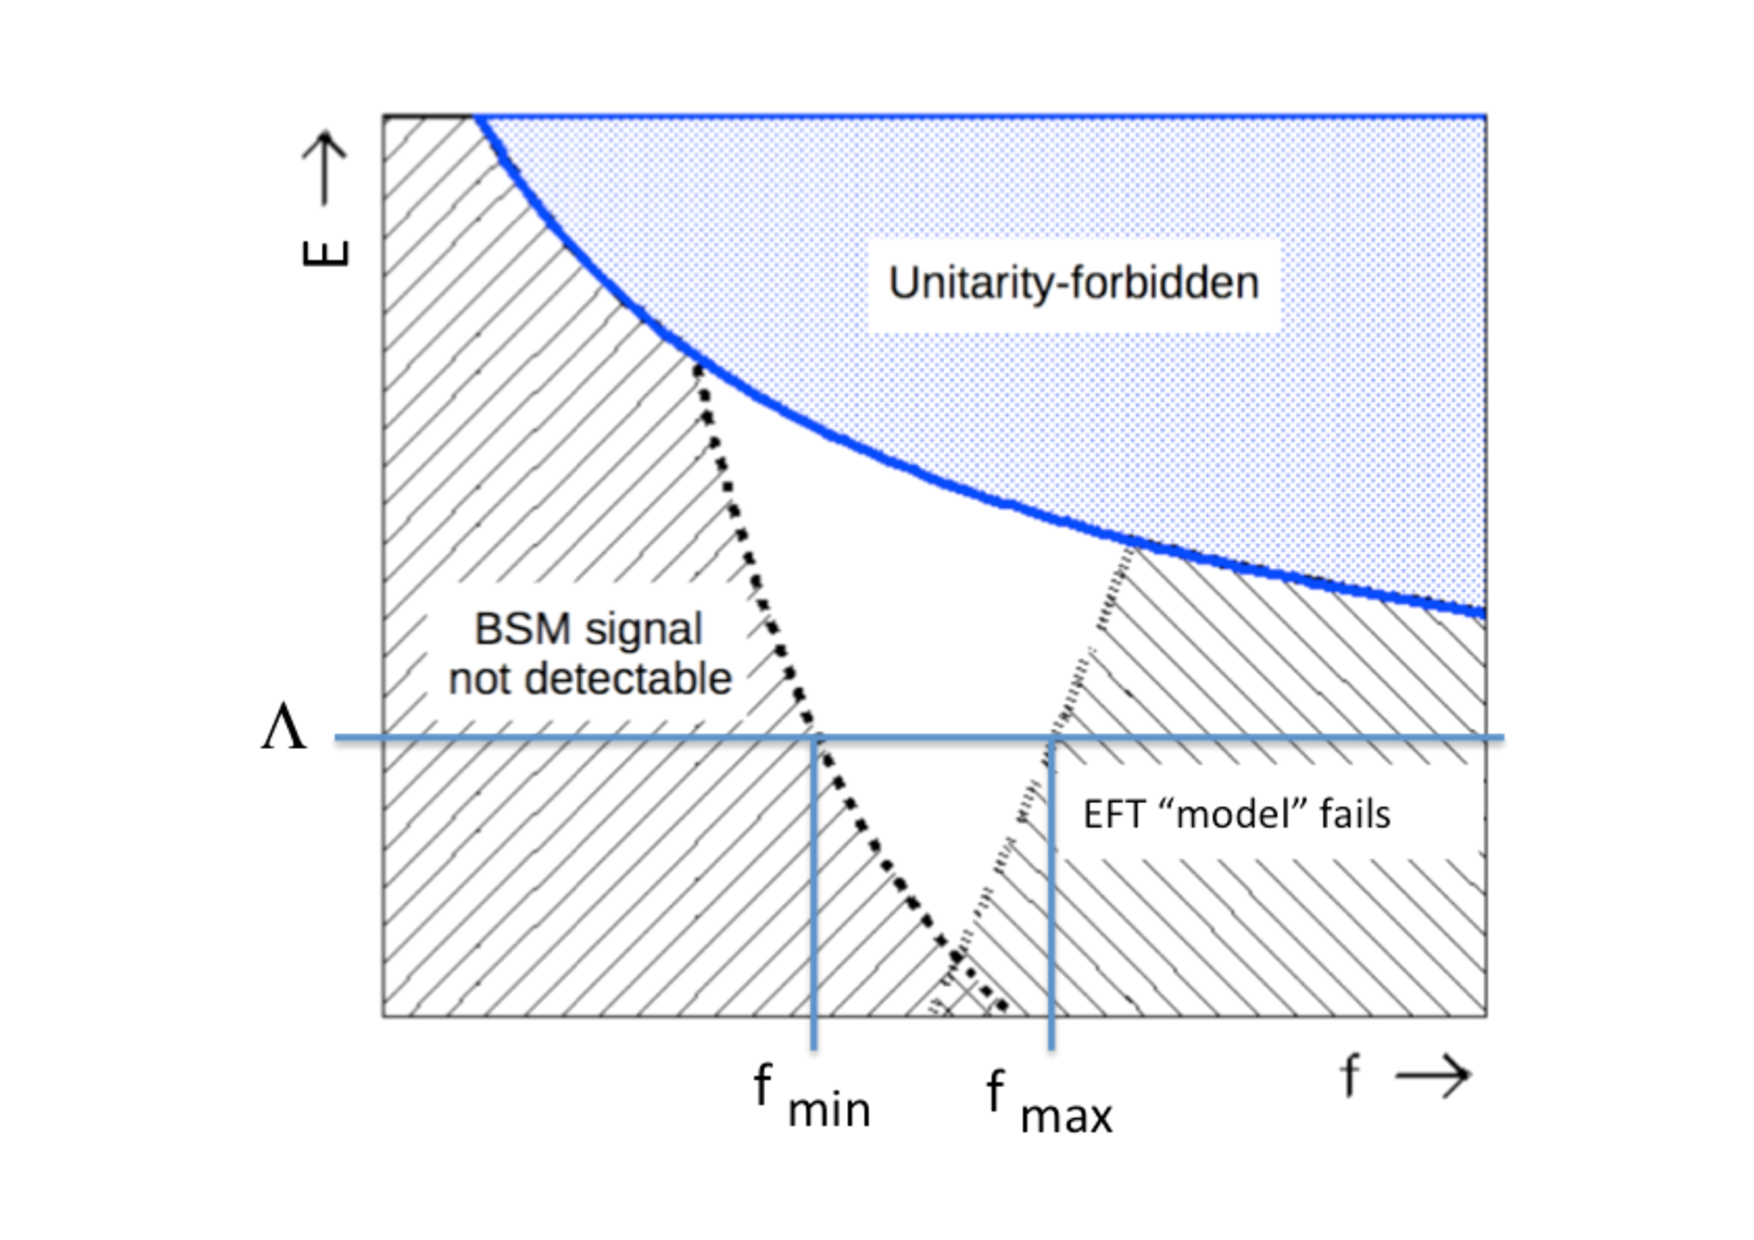
\includegraphics[width=0.8\linewidth]{\main/section4/plots/cartoon3.pdf}
\caption{
Cartoon plot showing the regions in $f_i$ and $\Lambda$ in terms of BSM signal observability
and applicability of the EFT ``model"  for  the same-sign WW process with purely 
leptonic decays.  The white triangle shows the region
where the BSM physics can be studied within the chosen EFT "model".}
%\vspace{1cm}
\label{fig:cartoonplot}
\end{figure}
%

For a given EFT ``model" the unitarity bound is very different for  different helicity amplitudes.
As  $M^U$ we take  the $lowest$ value from T-matrix diagonalisation of the $W^+W^+$ and $W^+W^-$, universally for all helicity 
amplitudes. 
The BSM signal  $S$ of the EFT ``model" $({\cal O}_i^{(d)},\,f_i^{(d)})$ 
can be defined as the deviation from SM predictions observed in the distribution of some observable $D$,  
$S=D^{model}-D^{SM}$.
A quantitative estimate of the signal can be written as
\small
\begin{equation} 
D^{model}=\int^{\Lambda}_{2M_W}\frac{d\sigma}{dM} \Bigl|_{model} dM +\int_{\Lambda}^{M_{max}}\frac{d\sigma}{dM}\Bigr|_{SM} dM\,,
\label{dsigma}
\end{equation}
\normalsize
which comes uniquely from the operator that defines the ``model" in its range
of validity and assumes only the SM contribution in the region $M>\Lambda$.
BSM contribution from the region above $\Lambda$   may enhance the signal, but it may also 
preclude proper description of the data in the EFT  "model",
which makes sense {\it if and only if} this additional contribution is small enough  
compared to the contribution from the validity region.  
For a  quantitative estimate of this 
contribution we define a second estimate in which  all the helicity amplitudes above 
$\Lambda$ are assumed to remain 
constant at their respective values they reach at $\Lambda$
\small
\begin{equation}
D^{model}=\int^{\Lambda}_{2M_W}\frac{d\sigma}{dM}\Bigl|_{model} dM +\int_{\Lambda}^{M_{max}}\frac{d\sigma}{dM}\Bigr|_{A=const} dM.
\label{unitarized}
\end{equation}
\normalsize
For $\Lambda = \Lambda_{max}$ this prescription regularises the helicity amplitudes that violate unitarity at $M^U$. 
We adopt the criterion that the EFT ``model" is tested for values of $(\Lambda\leq M^U, f_i)$ 
when the signals computed from Eq.(\ref{dsigma}) are statistically consistent 
within 2$\sigma$ with the signals computed with Eq.(\ref{unitarized}).

The observability of  the EFT "model" predictions imposes some minimum value of $f_{min}$, while the description within the EFT "model" imposes some 
maximum value of $f_{max}$ such that signal
estimates computed from Eqs.(\ref{dsigma}) and (\ref{unitarized}) remain 
statistically consistent.  
For $\Lambda=M^U$ a finite interval of $f_i$ values is possible, while 
for $\Lambda <M^U$ the  respective limits on $f_i$  depend on the actual value of $\Lambda$. It is illustrated in 
a cartoon plot in Fig.~\ref{fig:cartoonplot}, where the white "triangle" is bounded from 
above by the unitarity bound $M^U(f_i)$, from the left by the signal significance criterion 
and from the right by the consistency criterion.
The EFT "model" could be the right framework to describe the  BSM signal as long as the ``triangle"
shown in our cartoon plot is not empty.  






Our preferred strategy for data analysis is as follows:\\
a)  Measure  distributions $D$ that
offer the highest sensitivity to the studied EFT "model",\\
b) if deviations from the SM are observed, fit the values of 
$(\Lambda\leq M^U, f_i)$  according to 
Eq.(\ref{unitarized}),\\
c) using the fitted values of $f_i$ and $\Lambda$ recalculate 
$D$  templates 
according to 
Eq.(\ref{dsigma}),\\
d) check statistical consistency between estimates based on Eqs.(\ref{dsigma}) and (\ref{unitarized}). \\
 Physics conclusions from the obtained $(\Lambda, f_i)$ values can only be drawn
if such a consistency is found.  
%
%\begin{SCtable}[0.9][t]
%%\vspace{-2cm}
%\includegraphics[width=0.55\linewidth]{table.png}
%\caption{
%Estimated lower  and upper limits for BSM signal significance  for
%EFT consistency for each dimension-8 operator
%(positive and negative $f$ values), for the case when $\Lambda$ is equal
%to the unitarity bound,
%in the $W^+W^+$ scattering process at the LHC with 3 ab$^{-1}$.}
%%\vspace{1cm}
%\label{fig:cartoonplot}
%\end{SCtable}
%
Stability of the result against alternative 
regularisation methods  would provide a measure of uncertainty of the procedure - too much
sensitivity to the region above $\Lambda$ means the procedure is destined to fail
and  that data cannot be described within the chosen EFT "model".

%
%{\bf 3. Results of simulations.}  

To demonstrate our strategy we considered EFT ``models" defined by 
one-at-a-time dimension-8 operator that affects $WWWW$ couplings. Details of the simulation of events for  the process 
$pp \to jj\mu^+\mu^+\nu\nu$ (at 14 \UTeV with 3/ab integrated luminosity) and their processing according to our strategy can be found in \cite{Kalinowski:2018oxd}. 
Assuming $\Lambda$ equal to the respective unitarity bounds,
the lower and upper limits for the values of $f$ for each dimension-8 operator, for positive
and negative $f$ values, as well as the applicability "triangles" in the $(\Lambda,f_i)$ plane for each operator have been calculated.
  These limits define the (continuous) sets of testable 
EFT ``models" based on the choice of single dimension-8 operators. 


Following the above strategy we have calculated the expected reach for the dim-8 operator $O_{M7}$ at the HE-LHC and compared it with the obtained reach for the HL-LHC (14 \UTeV) from Ref.~\cite{Kalinowski:2018oxd}, assuming in each case an integrated luminosity of 3/ab.  Fig.\ref{fig:fM7} shows the respective ``EFT triangles".  It is evident that increasing the proton energy allows to explore much lower values of the Wilson coefficients, with lower limits for a 5$\sigma$ BSM discovery being shifted by as much as almost an order of magnitude.  On the other hand, the upper limit on consistent EFT description shifts likewise by a similar amount. This is due to the fact that by increasing the collision energy more and more events come from the region, where $M>\Lambda$ and therefore shrinking the range of Wilson coefficients that satisfy our consistency criterion.  Overall, the area of the actual ``EFT triangle" does not get significantly larger for 27 \UTeV compared to 14 \UTeV, even when viewed in a log scale.  

To summarise:  we have analysed the physics potential of "EFT models" defined by the choice of single dimension-8 operators in the same-sign WW scattering process in the purely leptonic decay modes.  
We argue that usage of EFT ``models" in the analysis of purely
leptonic $W$ decay channels requires bounding the possible contribution from
the region $M_{WW} > \Lambda$, no longer described by the ``model",
and ensuring it does not significantly distort the measured distributions 
compared to what they would have looked from the region of EFT validity alone and 
propose a data analysis strategy to satisfy the above requirements.  
We find that the "triangles"  turned to be rather narrow, even when going from 14 to 27 \UTeV of $pp$ beam energy . This result reinforces our former conclusion that study of BSM effects by means of varying single Wilson coefficients has little physics potential and future data analysis should be rather focused on simultaneous fits of many operators to the combined data from all VBS processes.  We find this conclusion to hold equally regardless of the actual beam energy.




\begin{figure}
\centering
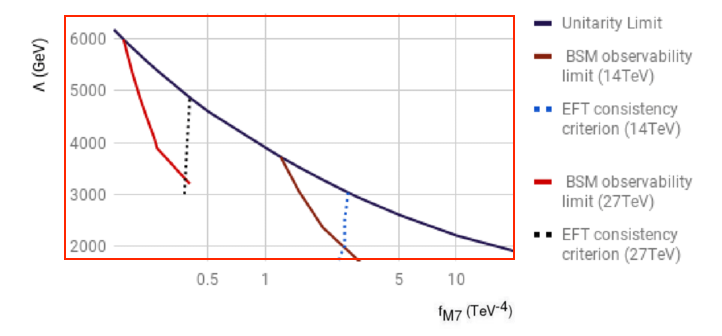
\includegraphics[width=0.7\linewidth]{\main/section4/plots/fM7.png}
\caption{
Regions in $f_{M7}$ and $\Lambda$ in terms of BSM signal observability
for the EFT ``model"  based on ${\cal O}_{M7}$ operator at the HL- and HE-LHC.}
%\vspace{1cm}
\label{fig:fM7}
\end{figure}




%
%%%%%%%%%%%%%%%%%%%%%%%%%
Acknowledgments: 
%%%%%%%%%%%%%%%%%%%%%%%%%
Work partially supported by the National Science Centre (Poland) grants
DEC-2015/18/M/ST2/00054,  DEC-2016/23/G/ST2/04301 (SP),
DEC-2015/19/B/ST2/02848 (JR) and 
HARMONIA project 
UMO-2015/18/M/ST2/00518  (JK) as well as the COST Action CA16108. 
ST is supported by Fermi Research Alliance, LLC under Contract No.~De-AC02-07CH11359 with the US DoE. The work of PK  has been supported by the Spanish MINECO project FPA2016-78220-C3-1- P (Fondos FEDER).
%%%%%%%%%%%%%%%%%%%%%%%%%
